\documentclass{classrep}
\usepackage[utf8]{inputenc}
\usepackage{color}
\usepackage{polski}
\usepackage{graphicx}

\DeclareUnicodeCharacter{00A0}{~}

\studycycle{Informatyka, studia dzienne, inż I st.}
\coursesemester{VI}

\coursename{Sztuczna inteligencja i systemy ekspertowe}
\courseyear{2019/2020}

\courseteacher{dr hab. inż. Piotr Lipiński}
\coursegroup{Poniedziałek, 12:00}

\author{
  \studentinfo{Maciej Pracucik}{216869} \and
  \studentinfo{Adam Jóźwiak}{216786}
}

\title{\textbf{Zadanie 2: Sieć neuronowa służąca do korygowania pomiaru systemu lokalizacji}}

\begin{document}
\maketitle

\section{Opis architektury sieci neuronowej}
{
	1. Liczba warstw sieci neuronowej - 5 (Jedna warstwa wejscia, trzy warstwy ukryte, jedna warstwa wyjścia) \\
	2. Liczebność neuronów w poszczególnych warstwach - 2, 30, 30, 30, 2 \\
	3. Funkcja aktywacji zastosowana w poszczególnych warstwach - RELU \\ (Rectified Linear Unit), która wyrażana jest wzorem y = max(0, x). Dla wszystkich wartości negatywnych przyjmuje wartość 0, natomiast dla wartości pozytywnych jest liniowa \\
	4. Liczba próbek z poprzednich chwil czasowych wykorzystywanych przez sieć neuronową - 80 \\
	5. Wagi poszczególnych neuronów w warstwach \\
 }

\section{Opis algorytmu uczenia sieci neuronowej}
{
	Algorytm używa klasy MLPRegressor z wysokopoziomowej biblioteki \\scikit-learn. Implementuje ona Multi-layer perceptron (MLP), który do nauki używa wstecznej propagacji, bez żadnej 
	funkcji aktywacji w warstwie wyjściowej. Do funckji straty wykorzystuje błąd kwadratowy, natomiast wynik działania sieci składa się z wartości stałych. \\
	Na początku dane z plików xlsx wczytywane są do jednego dużego datasetu, pobieramy z niego dane i dzielimy je na oczekiwane wyniki oraz dane wejściowe.
	Następnie dzielone są na dane testowe i treningowe.
	Do danych wejściowych, zarówno testowych jak i treningowych dodawane są punkty z poprzednich chwil czasowych, a w następnej kolejności dane te są skalowane za pomocą zewnętrznej klasy StandardScaler. Tworzymy model MLP z parametrami: ilość neuronów w warstwach ukrytych oraz ilość tych warstw, typ funkcji aktywacji, solver do optymalizacji wag, ilość iteracji oraz wizualne 		przedstawienie kolejnych iteracji wraz z wartością straty. Do utworzonego modelu przekazywane są dane treningowe wejściowe i wyjściowe. Następnie tworzone są predykcje z wykorzystaniem naszej sieci neuronowej, najpierw z wartościami treningowymi, a następnie dla wartości testowych. Odpowiednio dla  każdej z predykcji wyliczany jest błąd średniokwadratowy dla sprawdzenia 			poprawności i jakości sieci. Dla wizualizacji dane te są przedstawiane na wykresach.
}

\section{Porównanie dystrybuant błędu pomiaru}
{
	\begin{figure}[htp]
	\centering
	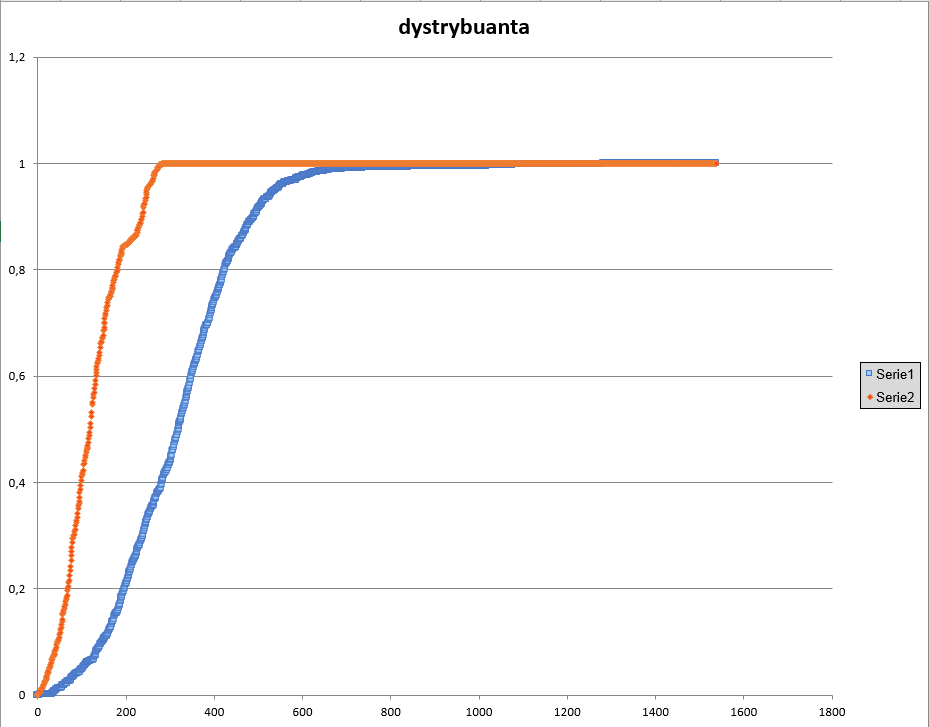
\includegraphics[width=15cm]{Wykres.png}
	\caption{Porównanie dystrybuant błędu pomiaru dla danych ze zbioru testowego oraz dla danych uzyskanych w wyniku filtracji przy użyciu sieci neuronowej. }
	\label{fig:lion}
	\end{figure}
	Dzięki wykresowi dystrybuant błędu, jesteśmy w stanie dowiedzieć się jakie są szanse, że błąd będzie mniejszy niż wartość błędu. W naszym przypadku, dzięki filtracji za pomocą sieci neuronowej uzyskaliśmy zdecydowanie mniejsze szanse na uzyskanie błędu. \\ 
	Weźmy przykładowe wartości, jeśli weźmiemy błąd np. 400 to przed filtracją mieliśmy 60\%, że błąd będzie co najwyżej 400, po filtracji jesteśmy w 100\% pewni, że błąd będzie poniżej 400. Weźmy inny przykład gdy dla błędu 200 nasze wyniki są w 100\% mniejsze lub równe 200, to przed filtracją mieliśmy szansę, że błąd będzie wiekszy niż 200.\\
	Dzięki filtracji przez sieć neuronową uzyskaliśmy dużo dokładniejsze wyniki, bliższe faktycznej pozycji robota.
}

\section{Kod źródłowy programu do uczenia i testowania sieci neuronowej}
{
	Zdecydowaliśmy się nie umieszczać kodu źródłowego, ponieważ wykorzystywaliśmy wysokopoziomowe biblioteki, przez co kod odpowiadający zarówno za uczenie jak i testowanie zajmuje 	bardzo mało linijek kodu.
}

\begin{thebibliography}{0}
  \bibitem{l2short} T. Oetiker, H. Partl, I. Hyna, E. Schlegl.
    \textsl{Nie za krótkie wprowadzenie do systemu \LaTeX2e}, 2007, dostępny
    online.
 \bibitem{scikit}Dokumentacja biblioteki Scikit - Learn
	\textsl{\url{https://scikit-learn.org/}}
\bibitem{pluralsight} Pluralsight - tutorial
	\textsl{ \url{https://www.pluralsight.com/guides/machine-learning-neural-networks-scikit-learn}}
\end{thebibliography}

\end{document}
